\documentclass[a4paper,10pt, twocolumn]{article}
\usepackage[german, english]{babel} % Languages
\usepackage{tikz} % Tikz figures
\usepackage{siunitx} % SI-units package
\usepackage{bm} % Bold mathematics
\usepackage{listings} % Make listings, e.g. for code
\usepackage{enumitem} % Enumerate and itemize commands
\usepackage{multicol} % Make multiple columns for content
\usepackage[left=15mm, right=15mm, bottom=15mm, top=15mm, includeheadfoot]{geometry} % Modify geometry of page format
\usepackage{placeins} % For float barrier command
\usepackage{amsmath} % Math environments
\usepackage{fancyhdr} % Include the fancyhdr package
\usepackage{amsthm} % Theorem environments
\usepackage{siunitx} % Use SI
\usepackage{array} % Use array package for tables
\usepackage{tabularx} % Package to make nice tables
\usepackage{amssymb} % Math symbols
\usepackage{lipsum} % Provide dummy text
\usepackage{abstract} % Abstract package
\usepackage{nicefrac} % Nice fractions in in-line texts
\usepackage[hidelinks]{hyperref} % Make document with hyperlinks
\usepackage{cleveref} % Make references
\usepackage{subcaption} % Make subfigures
\usepackage{graphicx} % Make figures
\usepackage{mhchem} % Chemical notation
\usepackage{mathtools} % Various math tools
\usepackage{framed} % Frame equations
% Figure caption setup
\captionsetup{font=footnotesize,labelfont=bf}

% Python code listings
\definecolor{codegreen}{rgb}{0,0.6,0}
\definecolor{codegray}{rgb}{0.5,0.5,0.5}
\definecolor{codepurple}{rgb}{0.58,0,0.82}
\definecolor{backcolour}{rgb}{0.95,0.95,0.92}

\lstdefinestyle{mystyle}{
	backgroundcolor=\color{backcolour},   
	commentstyle=\color{codegreen},
	keywordstyle=\color{magenta},
	numberstyle=\tiny\color{codegray},
	stringstyle=\color{codepurple},
	basicstyle=\ttfamily\footnotesize,
	breakatwhitespace=false,         
	breaklines=true,                 
	captionpos=b,                    
	keepspaces=true,                 
	numbers=left,                    
	numbersep=5pt,                  
	showspaces=false,                
	showstringspaces=false,
	showtabs=false,                  
	tabsize=2
}

% Enumerate style
\renewcommand{\theenumi}{(\arabic{enumi})}
\renewcommand\labelenumi{\theenumi} % Change enumerate style from 1. to (1) etc.
\renewcommand{\theenumiii}{(\arabic{enumiii})}
\renewcommand\labelenumiii{\theenumiii} % Change enumerate style from 1. to (1) etc.
\setlist{itemsep = 0.2pt}

% Matrix and vector notation
\newcommand\matr[1]{\ensuremath{\boldsymbol{\mathbf{#1}}}}
\newcommand\vect[1]{\ensuremath{\bm{#1}}}
\newcommand\dint{\ensuremath{\int\displaylimits}}

% Units definitions
\DeclareSIUnit \parsec {pc}
\DeclareSIUnit \magnitudes {mag}

% Theorem environment
\newtheorem{tm}{Theorem}
\numberwithin{tm}{subsection}

% New tag form
\newtagform{normalsize}[\normalsize]{\normalsize(}{\normalsize)}

% Configure head- and footlines
\pagestyle{fancy} % Set head- and footlines
\fancyhead[C]{Adult face predicting machine} % Left headline
\fancyhead[L]{\nouppercase{\leftmark}} % Right headline
\fancyhead[R]{D. Zahnd, R. Zahnd}

\author{Daniel Zahnd, Regula Zahnd}
\date{August 28, 2024 - \today}
\title{Adult face predicting machine \\ \vspace{0.5cm} \normalsize Theory and test report on an AI model predicting an adult face based on the image of a baby face}

\begin{document}

\maketitle


\begin{abstract}
Text.
\end{abstract}

\section{Introduction}
Introduction to the topic at hand; and explain, why it is to be solved using deep learning models.

\section{Theoretical foundation}
\subsection{Background}
Give some background on the topic at hand, and by what tools it is to be solved.

\subsection{Neural networks}
Introduce neural networks as the basic building block of any deep learning model.

\subsubsection{Single layer perceptron}
Explain theory on single layer perceptron.

\subsubsection{Multi layer perceptron}
Explain theory on multi layer perceptrons.

\subsubsection{Loss function}
Explain, why a loss function is needed for an SLP or MLP.

\subsubsection{Training process}
Explain how one goes about training a deep learning model.

\subsection{Convolutional neural networks}
Exlain the working principle of convolutional neural networks and why they are effective at machine vision tasks.

\subsection{Generative models}
Explain, what generative models in deep learning are. Mention the three basic generative models; GAN's, VAE's and flows. Explain, why GAN's are to be used for the task at hand and why the other models are not suitable for the task.

\subsubsection{Generative adversarial networks (GAN)}
%Explain theory on GAN's.
Generative adversarial networks function as sketched in \cref{fig:GAN}. A generative adversarial network consists of a generator and a discriminator. The generator is basically a function $\bar{\vect{x}} = \vect{G}_{\vect{\phi}}(\vect{z})$, where $\bar{\vect{x}}$ is the output of the generator, $\vect{\phi}$ are the weights associated to the neural network implementing the generator function and $\vect{z}$ is a latent variable, which is chosen to follow a standard normal distribution, i.e. $\vect{z} \sim p_{\vect{z}}(\vect{z}) = \mathcal{N}(0,1)^d$ with $d \in \mathbb{N}$ again the dimensionality of the latent space. The purpose of the generator is to generate fake data $\bar{\vect{x}}$ based on samples $\vect{z}$ of the latent probability density $p_{\vect{z}}(\vect{z})$. The discriminator however takes an input $\vect{x}$, such as the output of the generator, and outputs a value 0 or 1, where 0 stands for ``input is fake'' and 1 represents the situation ``input is real''. The task of the discriminator is therefore to decide, if an input $\vect{x}$ is fake or real.
\begin{figure}[h!]
	\centering
	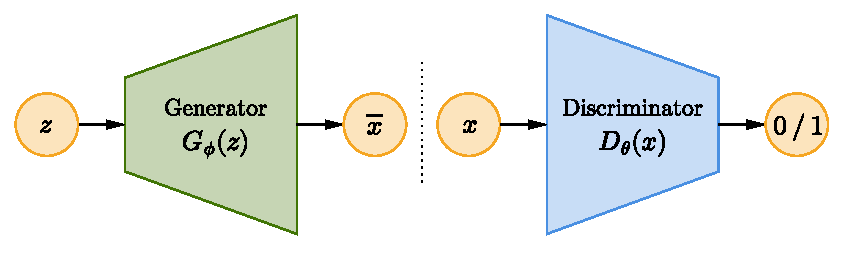
\includegraphics[width=0.4\textwidth]{figures/GAN.pdf}
	\caption{Working principle of a generative adversarial network (GAN). Figure inspired by \cite{weng2018flow}.}
	\label{fig:GAN}
\end{figure}

A generative adversarial network is trained in such a way, that the generator learns how to generate the best possible real-looking data $\bar{\vect{x}}$, whereas the discriminator learns as good as possible to distinguish between real data contained in the training set $\hat{\matr{x}}$ and fake data $\bar{\vect{x}}$ generated by the generator. Herein lies the adversarity of the model; the generator and the discriminator are actually competing against each other; the generator learns how to create the best possible fake data, whereas the discriminator learns, how to best distinguish between real and fake data - in this way, both the generator and the discriminator are optimized for their respective task. The loss function for training therefore has to be defined accordingly in a game-theoretical manner, where both the discriminator and the generator try to optimize their outcomes. Once trained, one can just use the generator to create fake data $\bar{\vect{x}} = \vect{G}_{\vect{\phi}}(\vect{z})$ from samples $\vect{z}$ of $p_{\vect{z}}(\vect{z})$ at will.

\subsubsection{Conditional generative adversarial networks (cGAN)}
Explain theory on cGAN's.


\section{Methods}
\subsection{GAN on the MNIST dataset}
Explain methods for a GAN on the MNIST dataset.

\subsection{GAN on faces dataset}
Explain methods for a GAN on a faces dataset.

\subsection{cGAN on MNIST dataset}
Explain methods for cGAN's on the MNIST dataset.

\subsection{cGAN (Pix2Pix) on baby face photo dataset)}
Explain methods for cGAN's on the baby face photo dataset.

\section{Results}
\subsection{GAN on the MNIST dataset}
Explain results for a GAN on the MNIST dataset.

\subsection{GAN on faces dataset}
Explain results for a GAN on a faces dataset.

\subsection{cGAN on MNIST dataset}
Explain results for cGAN's on the MNIST dataset.

\subsection{cGAN (Pix2Pix) on baby face photo dataset)}
Explain results for cGAN's on the baby face photo dataset.

\section{Discussion}
\subsection{GAN on the MNIST dataset}
Discuss results for a GAN on the MNIST dataset.

\subsection{GAN on faces dataset}
Discuss results for a GAN on a faces dataset.

\subsection{cGAN on MNIST dataset}
Discuss results for cGAN's on the MNIST dataset.

\subsection{cGAN (Pix2Pix) on baby face photo dataset)}
Discuss results for cGAN's on the baby face photo dataset.

\section{Conclusions}
Draw general conclusions from the conducted experiments and their outcomes.

\appendix
\section{Appendix 1}
Elucidate on possible appendices.


\nocite{goodfellow2014generativeadversarialnetworks}
\nocite{isola2018imagetoimagetranslationconditionaladversarial}
\nocite{DBLP:journals/corr/MirzaO14}

\bibliography{references}
\bibliographystyle{apalike}

\end{document}